\section {Implementation and Technical Notes}

Python 3.6 was used to code, with modularity of components being the main focus. \\

The code has been split into modules as per the required question


\section {Question 1}

We use \textit{scikit} to perform PCA, and \textit{pytorch } to train linear and deep auto-encoder models.

\begin{lstlisting}

\end{lstlisting}

The code to train the model is:

\begin{lstlisting}
python3 q1.py 
\end{lstlisting}

\begin{itemize}
\item Learning rate of $1e-3$, with Adam was used as the optimiser.
\item We periodically run evaluation post an epoch. 
\item Loss is MSE with respect to reconstruction.
\end{itemize}

\subsection{Accuracy and Loss Plots}

We report MSE loss convergence for the autoencoder models, along with their image reconstructions.

We observe the following:

\begin{itemize}
\item The linear autoencoder performs comparatively to PCA, however, with a different latent space representation. This is intuitive, since a PCA is the best fit linear transform, and if the network were optimal, it would mimic PCA.
\item  The deep autoencoder does much better than PCA, and has less than $1e-3$ MSE error when trained for more than 12 epochs (batch size 256). This is due to the fact that manifold learning, and not necessarily a linear transformation can occur.
\end{itemize}
\begin{figure}[!htbp]
          \begin{subfigure}
          \centering
          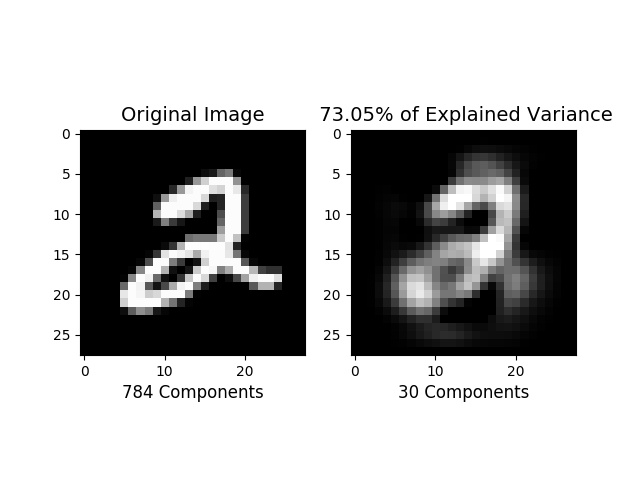
\includegraphics[angle=0,width=0.65\textwidth]{assign-4/logs/q1/pca.png}
          \caption{PCA Reconstruction, 30 components.}
          \end{subfigure}
          \end{figure}

\begin{figure}[!htbp]
          \begin{subfigure}
          \centering
          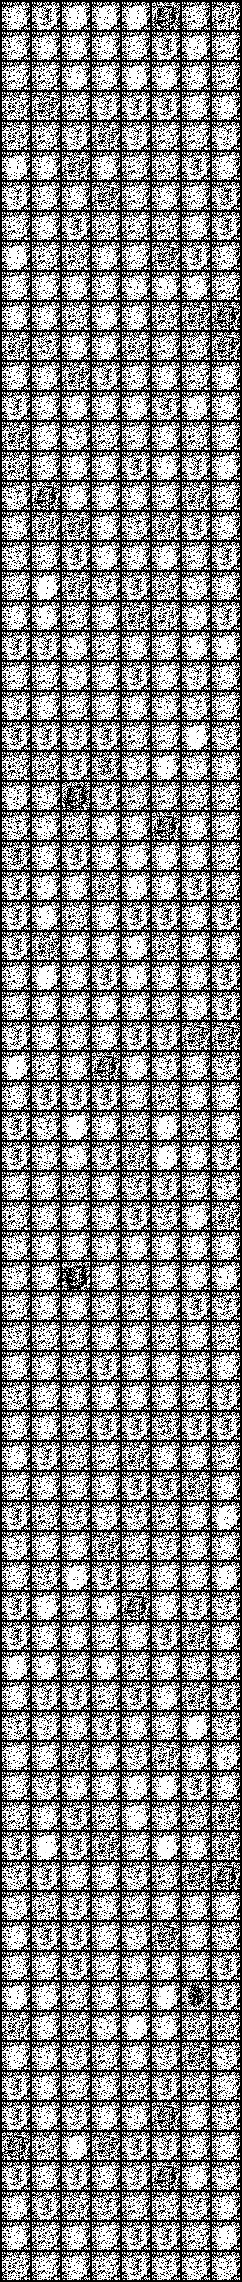
\includegraphics[angle=0,width=0.65\textwidth]{assign-4/logs/q1/linear_autoencoder/image_90.png}
          \caption{Linear Autoencoder, 1000 - 500 - 250 - 30 - 250 - 500 - 1000, reconstruction}
          \end{subfigure}
          \begin{subfigure}
          \centering
          \includegraphics[angle=0,width=0.65\textwidth]{assign-4/logs/q1/image-90.png}
          \caption{MSE Loss training convergence}
          \end{subfigure}
          \end{figure}
          
          \begin{figure}[!htbp]
          \begin{subfigure}
          \centering
          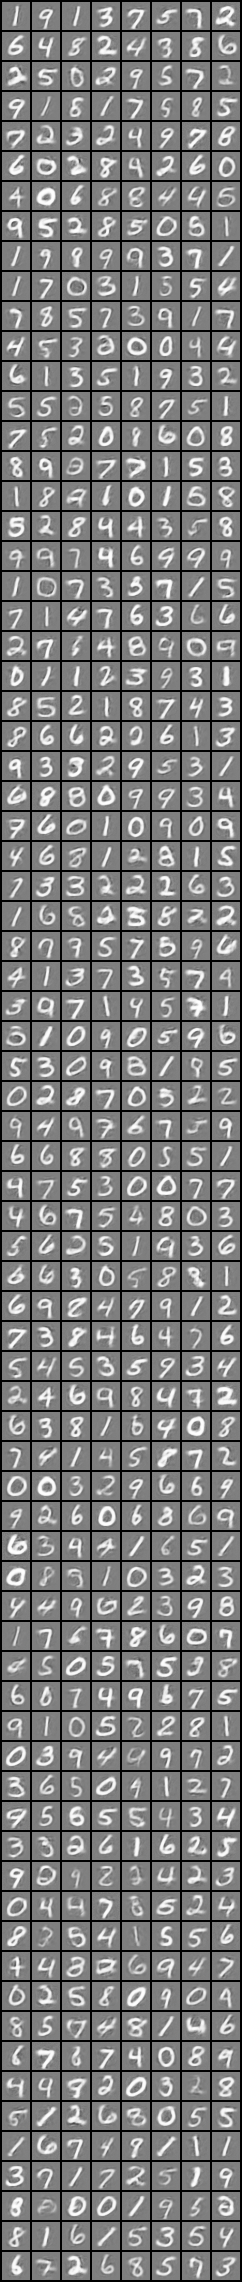
\includegraphics[angle=0,width=0.65\textwidth]{assign-4/logs/q1/deep_autoencoder/image_90.png}
          \caption{Deep Autoencoder, 1000 - 500 - 250 - 30 - 250 - 500 - 1000, reconstruction}
          \end{subfigure}
          \begin{subfigure}
          \centering
          \includegraphics[angle=0,width=0.65\textwidth]{assign-4/logs/q1/image-90.png}
          \caption{MSE Loss training convergence}
          \end{subfigure}
          \end{figure}




\section{Question 2 }

We design a standard Auto-encoder, with once hidden unit and experiment for various hidden units, of sizes: [64,128,256,512]. 
\end{itemize}

The outputs of this question may be generated by:
\begin{lstlisting}
python3 q2.py 
\end{lstlisting} 

We notice that increasing the hidden unit size increases the accuracy of reconstruction, due to better representation power.

\subsection{Loss and Accuracy Curves for H values}

\begin{figure}[!htbp]
          \begin{subfigure}
          \centering
          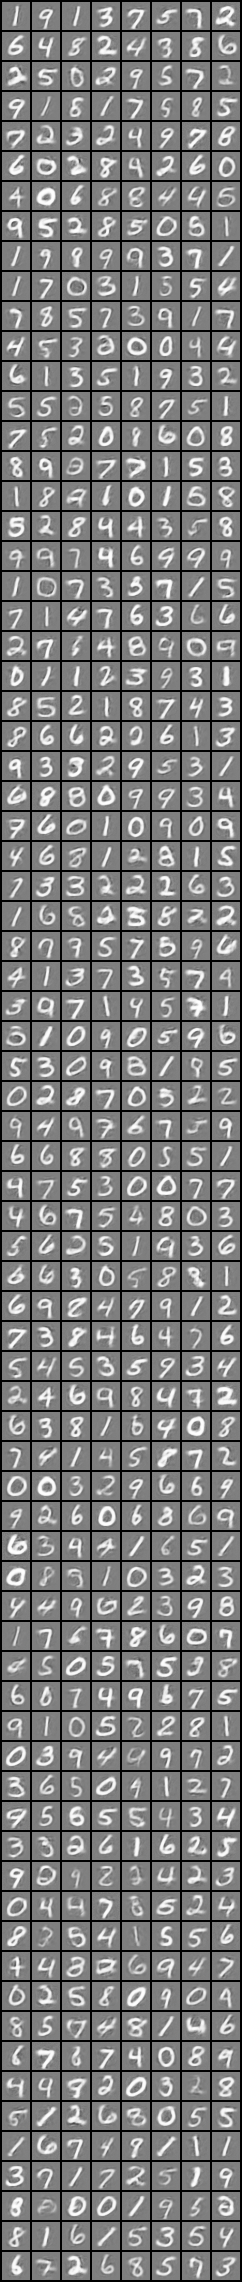
\includegraphics[angle=0,width=0.65\textwidth]{assign-4/logs/q1/deep_autoencoder/image_90.png}
          \caption{Deep Autoencoder, 1000 - 500 - 250 - 30 - 250 - 500 - 1000, reconstruction}
          \end{subfigure}
          \begin{subfigure}
          \centering
          \includegraphics[angle=0,width=0.65\textwidth]{assign-4/logs/q1/image-90.png}
          \caption{MSE Loss training convergence}
          \end{subfigure}
          \end{figure}
          \begin{figure}[!htbp]
          \begin{subfigure}
          \centering
          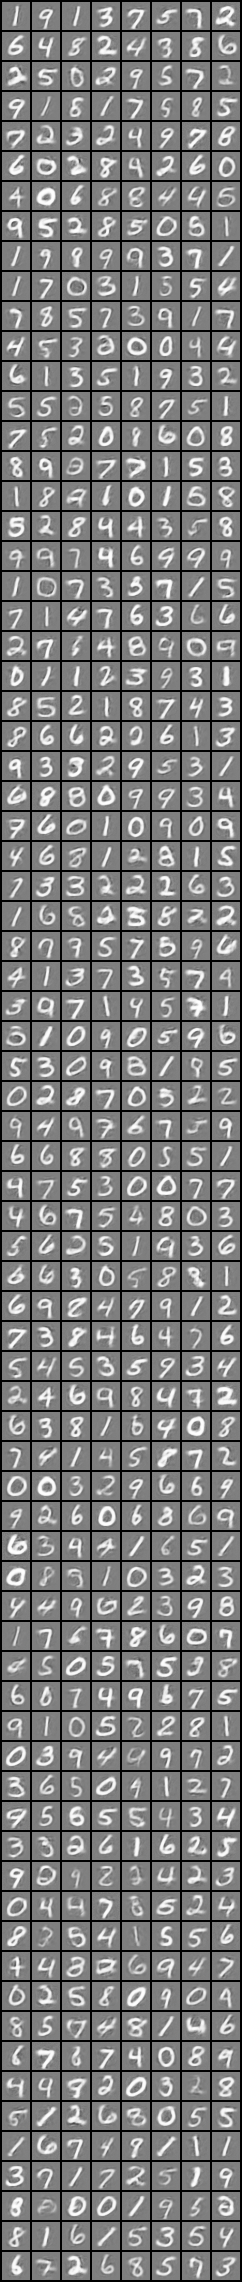
\includegraphics[angle=0,width=0.65\textwidth]{assign-4/logs/q1/deep_autoencoder/image_90.png}
          \caption{Deep Autoencoder, 1000 - 500 - 250 - 30 - 250 - 500 - 1000, reconstruction}
          \end{subfigure}
          \begin{subfigure}
          \centering
          \includegraphics[angle=0,width=0.65\textwidth]{assign-4/logs/q1/image-90.png}
          \caption{MSE Loss training convergence}
          \end{subfigure}
          \end{figure}
          
          \begin{figure}[!htbp]
          \begin{subfigure}
          \centering
          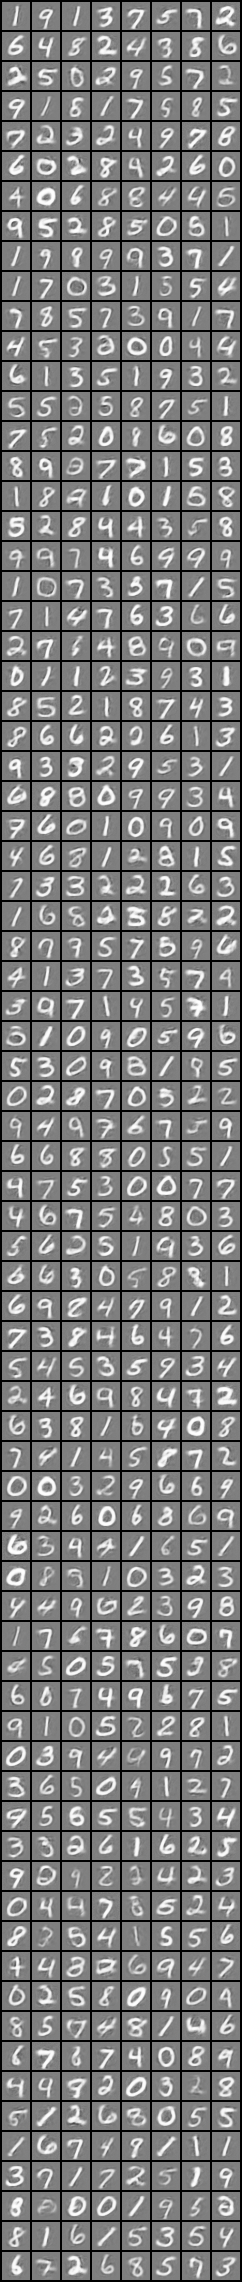
\includegraphics[angle=0,width=0.65\textwidth]{assign-4/logs/q1/deep_autoencoder/image_90.png}
          \caption{Deep Autoencoder, 1000 - 500 - 250 - 30 - 250 - 500 - 1000, reconstruction}
          \end{subfigure}
          \begin{subfigure}
          \centering
          \includegraphics[angle=0,width=0.65\textwidth]{assign-4/logs/q1/image-90.png}
          \caption{MSE Loss training convergence}
          \end{subfigure}
          \end{figure}
          
       \begin{figure}[!htbp]
          \begin{subfigure}
          \centering
          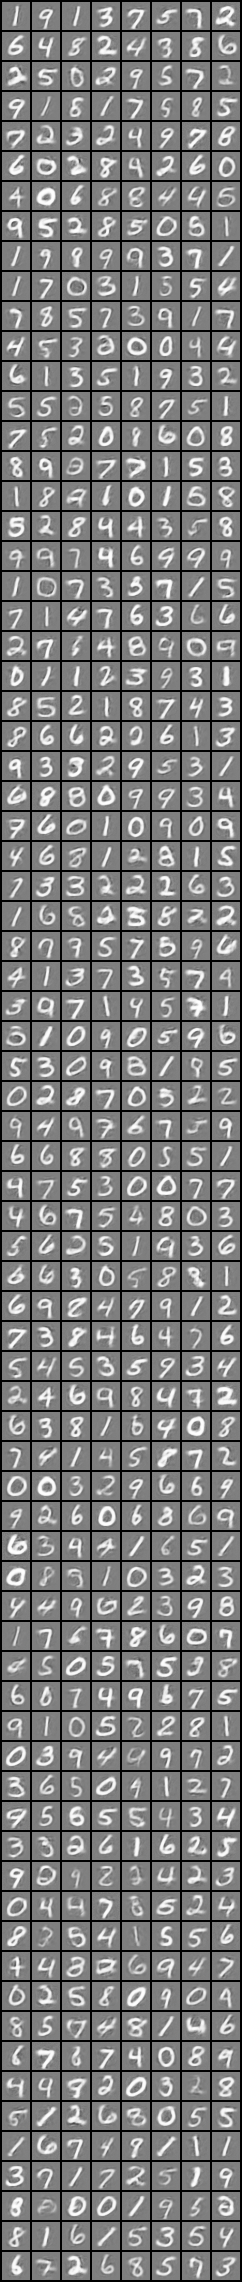
\includegraphics[angle=0,width=0.65\textwidth]{assign-4/logs/q1/deep_autoencoder/image_90.png}
          \caption{Deep Autoencoder, 1000 - 500 - 250 - 30 - 250 - 500 - 1000, reconstruction}
          \end{subfigure}
          \begin{subfigure}
          \centering
          \includegraphics[angle=0,width=0.65\textwidth]{assign-4/logs/q1/image-90.png}
          \caption{MSE Loss training convergence}
          \end{subfigure}
          \end{figure}
          

\section{Question 3}

We implement sparsity by pytorch's L1 weight penalisation, over the latent representation.

The outputs of this question may be generated by:

\begin{lstlisting}
python3 q3.py --loss_type MSE
\end{lstlisting} 

Hyper-parameters:
\begin{itemize}
\item  Adam optimiser, lr = 0.01, beta1 = 0.9, beta2 = 0.99
\item  Loss : MSE and Cross Entropy
\item  Single hidden layer, 5 units wide.
\end{itemize}

\subsection{MSE vs Cross Entropy}

We also note that MSE performs much better than Cross Entropy. This is because the output sequence is a binary number and their probabilities are correlated. Hence, we cannot use a "clean" version of cross entropy with $L$ distinct distributions. We use a hackish method to use cross entropy, and for the reasons noted above, it performs poorly. We plot validation in blue, train in orange.

\begin{figure}[!htbp]
\begin{subfigure}
\centering
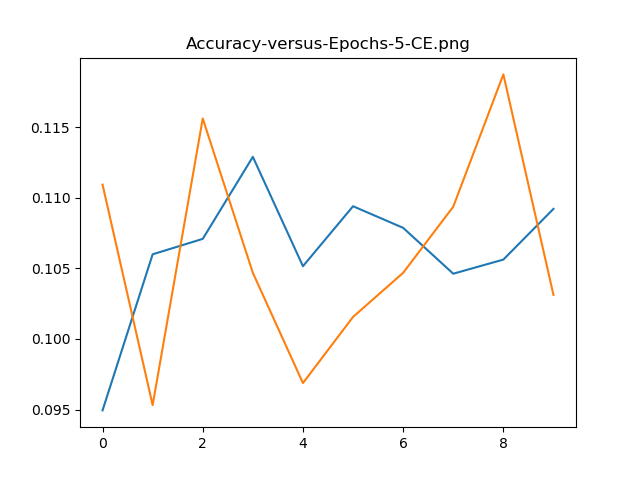
\includegraphics[angle=0,width=0.65\textwidth]{assign-3/logs/Accuracy-5-CE-hidden-5.png}
\caption{$L=5$, Cross Entropy Loss}
\end{subfigure}
\begin{subfigure}
\centering
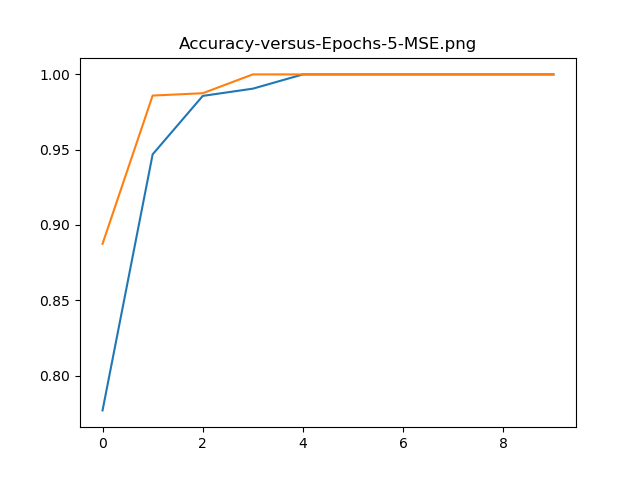
\includegraphics[angle=0,width=0.65\textwidth]{assign-3/logs/Accuracy-5-MSE-hidden-5.png}
\caption{$L=5$, MSE Loss}
\end{subfigure}
\end{figure}

\begin{figure}[!htbp]
\begin{subfigure}
\centering
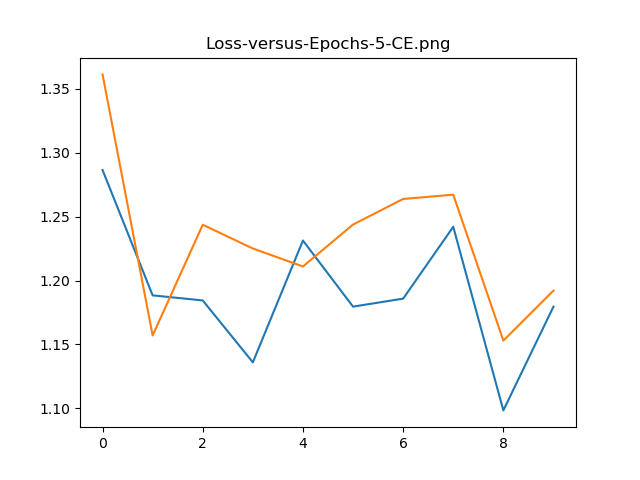
\includegraphics[angle=0,width=0.65\textwidth]{assign-3/logs/Loss-5-CE-hidden-5.png}
\caption{$L=5$, Cross Entropy Loss}
\end{subfigure}
\begin{subfigure}
\centering
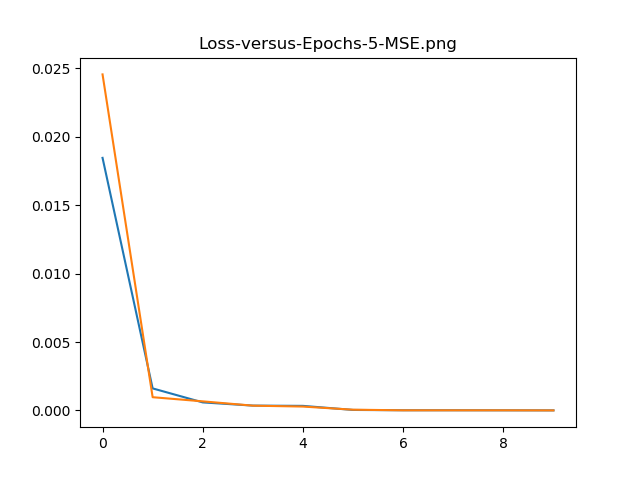
\includegraphics[angle=0,width=0.65\textwidth]{assign-3/logs/Loss-5-MSE-hidden-5.png}
\caption{$L=5$, MSE Loss}
\end{subfigure}
\end{figure}

\subsection{MSE: Loss and Accuracy Curves}

We include loss and accuracy curves for all sequence lengths (3,5,10) used.

\begin{figure}[!htbp]
\begin{subfigure}
\centering
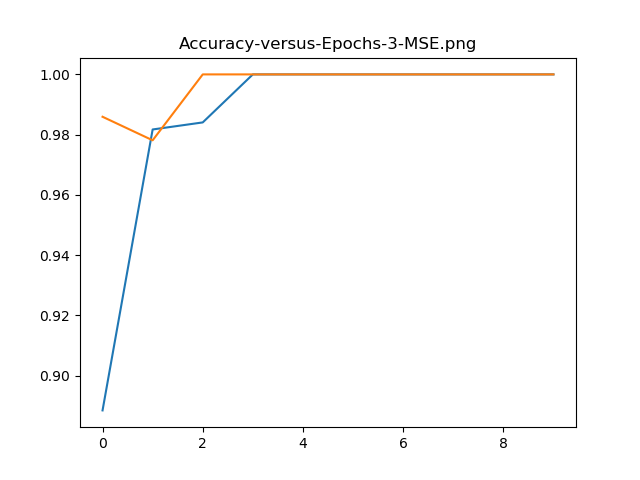
\includegraphics[angle=0,width=0.65\textwidth]{assign-3/logs/Accuracy-3-MSE-hidden-5.png}
\caption{$L=3$, Accuracy, MSE}
\end{subfigure}
\begin{subfigure}
\centering
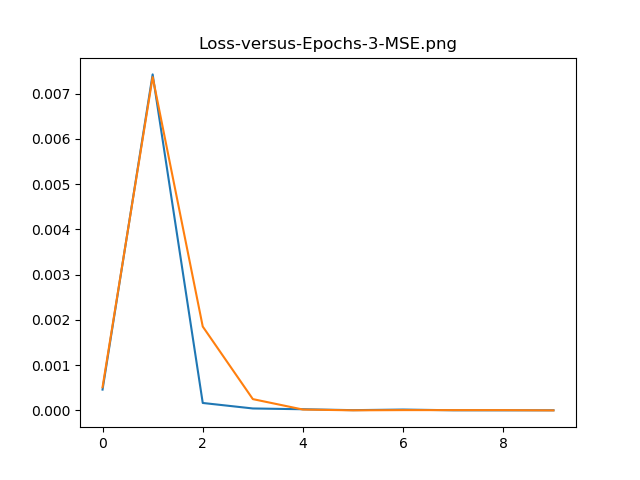
\includegraphics[angle=0,width=0.65\textwidth]{assign-3/logs/Loss-3-MSE-hidden-5.png}
\caption{$L=3$, Loss , MSE}
\end{subfigure}
\end{figure}

\begin{figure}[!htbp]
\begin{subfigure}
\centering
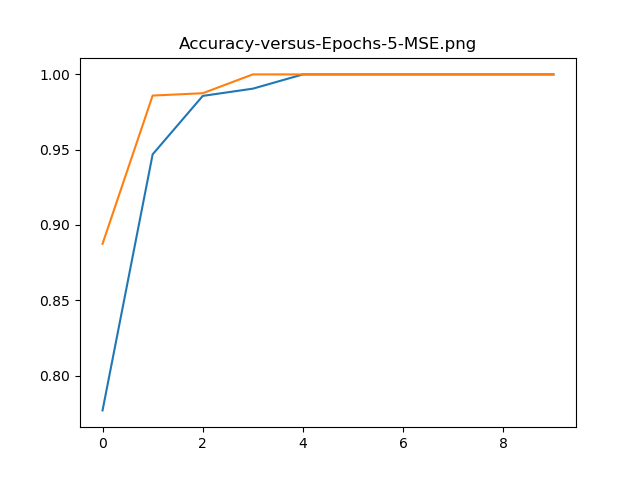
\includegraphics[angle=0,width=0.65\textwidth]{assign-3/logs/Accuracy-5-MSE-hidden-5.png}
\caption{$L=5$, Accuracy, MSE}
\end{subfigure}
\begin{subfigure}
\centering
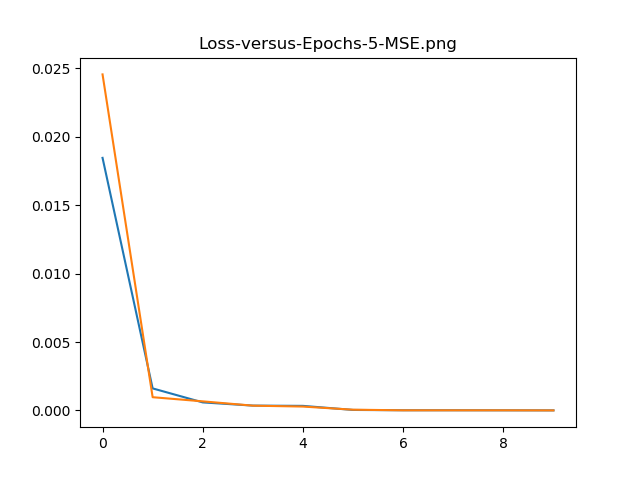
\includegraphics[angle=0,width=0.65\textwidth]{assign-3/logs/Loss-5-MSE-hidden-5.png}
\caption{$L=5$, Loss, MSE}
\end{subfigure}
\end{figure}

\begin{figure}[!htbp]
\begin{subfigure}
\centering
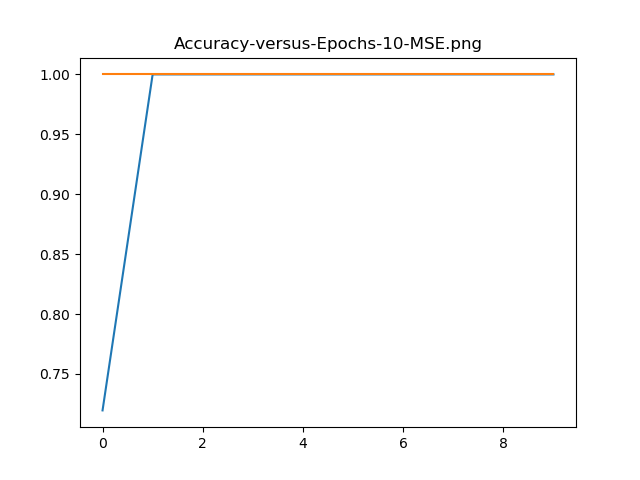
\includegraphics[angle=0,width=0.65\textwidth]{assign-3/logs/Accuracy-10-MSE-hidden-5.png}
\caption{$L=10$, Accuracy, MSE}
\end{subfigure}
\begin{subfigure}
\centering
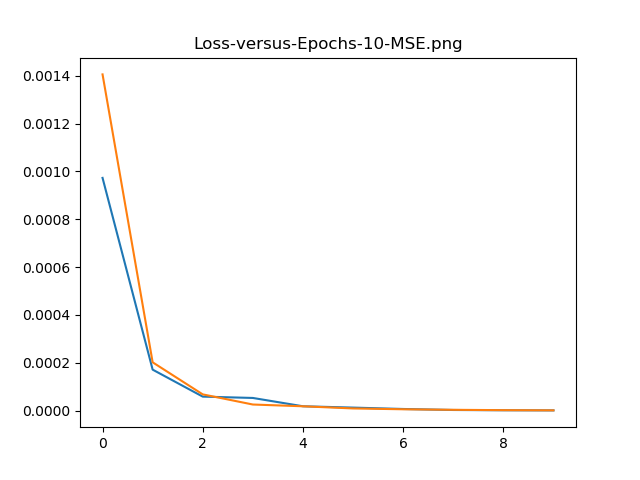
\includegraphics[angle=0,width=0.65\textwidth]{assign-3/logs/Loss-10-MSE-hidden-5.png}
\caption{$L=10$, Loss, MSE}
\end{subfigure}
\end{figure}

\subsection{MSE: Average Bit accuracy}

We perform this for $L=3, 5, 10$ as the training data.

\begin{figure}[!htbp]
\begin{subfigure}
\centering
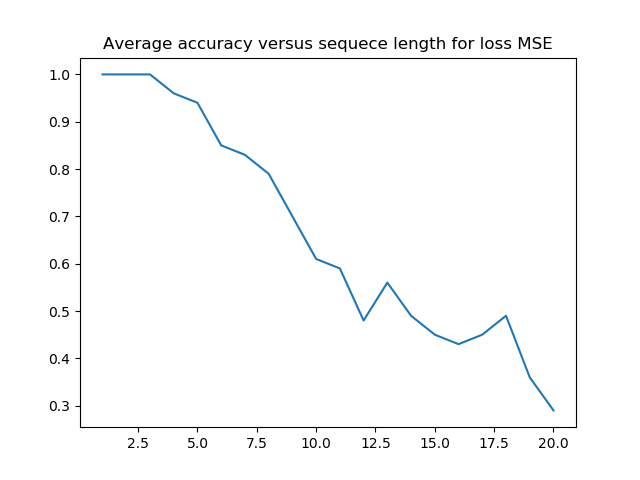
\includegraphics[angle=0,width=0.65\textwidth]{assign-3/logs/AV-Loss-3-MSE-hidden-5.png}
\caption{$L=3$, Average Bit rate Loss}
\end{subfigure}
\begin{subfigure}
\centering
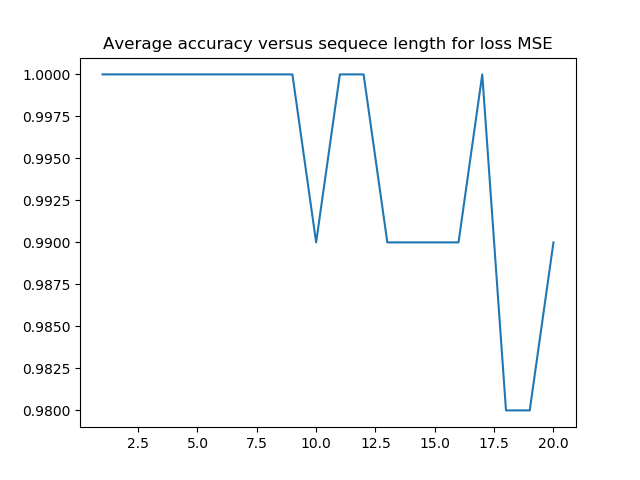
\includegraphics[angle=0,width=0.65\textwidth]{assign-3/logs/AV-Loss-5-MSE-hidden-5.png}
\caption{$L=5$, Average Bit rate Loss}
\end{subfigure}
\begin{subfigure}
\centering
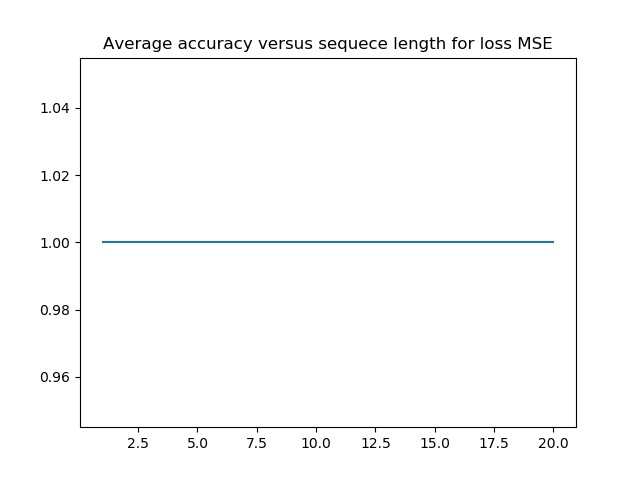
\includegraphics[angle=0,width=0.65\textwidth]{assign-3/logs/AV-Loss-10-MSE-hidden-5.png}
\caption{$L=10$, Average Bit rate Loss}
\end{subfigure}
\end{figure}






 